% $Id$
%
% Earth System Modeling Framework
% Copyright 2002-2013, University Corporation for Atmospheric Research, 
% Massachusetts Institute of Technology, Geophysical Fluid Dynamics 
% Laboratory, University of Michigan, National Centers for Environmental 
% Prediction, Los Alamos National Laboratory, Argonne National Laboratory, 
% NASA Goddard Space Flight Center.
% Licensed under the University of Illinois-NCSA License.

The ESMF Grid class is used to describe the geometry and discretization
of logically rectangular physical grids.  It also contains the
description of the grid's underlying topology and the decomposition
of the physical grid across the available computational resources.
The most frequent use of the Grid class is to describe physical grids
in user code so that sufficient information is available to perform ESMF
methods such as regridding.  

%In the current release (v5.2.0)
%the functionality in this class is partially implemented.  
%Multi-tile grids are not supported, and edge connectivities 
%are not implemented and default to aperiodic.  
%Other constraints of the current
%implementation are noted in the usage section and in the API
%descriptions.


\begin{center}
\begin{tabular}{|p{6in}|}
\hline
\vspace{.01in}
{\bf Key Features} \\[.01in]
Representation of grids formed by logically rectangular regions,
including uniform and rectilinear grids (e.g. lat-lon grids),
curvilinear grids (e.g. displaced pole grids), and grids formed
by connected logically rectangular regions (e.g. cubed sphere grids).\\
Support for 1D, 2D, 3D, and higher dimension grids.\\ 
Distribution of grids across computational resources for parallel
operations - users set which grid dimensions are distributed.\\
Grids can be created already distributed, so that no single
resource needs global information during the creation process.\\
Options to define periodicity and other edge connectivities either 
explicitly or implicitly via shape shortcuts.\\ 
Options for users to define grid coordinates themselves or call
prefabricated coordinate generation routines for standard grids
[NO GENERATION ROUTINES YET].\\
Options for incremental construction of grids.\\
Options for using a set of pre-defined stagger locations or for setting
custom stagger locations.\\ [.03in] \hline
\end{tabular}
\end{center}

\subsubsection{Grid Representation in ESMF}

ESMF Grids are based on the concepts described in {\it A Standard
Description of Grids Used in Earth System Models} [Balaji 2006].  In this document
Balaji introduces the mosaic concept as a means of describing
a wide variety of Earth system model grids.  A {\bf mosaic} is
composed of grid tiles connected at their edges.  Mosaic grids
includes simple, single tile grids as a special case.  

The ESMF Grid class is a representation of a mosaic grid.  Each ESMF
Grid is constructed of one or more logically rectangular {\bf Tiles}.
A Tile will usually have some physical significance (e.g. the region
of the world covered by one face of a cubed sphere grid).

The piece of a Tile that resides on one DE (for simple cases, a DE
can be thought of as a processor - see section on the DELayout)
is called a {\bf LocalTile}.  For example, the six faces of a cubed
sphere grid are each Tiles, and each Tile can be divided into many
LocalTiles.  

Every ESMF Grid contains a DistGrid object, which defines the Grid's
index space, topology, distribution, and connectivities.  It enables
the user to define the complex edge relationships of tripole and other
grids.  The DistGrid can be created explicitly and passed into a Grid
creation routine, or it can be created implicitly if the user takes
a Grid creation shortcut. The DistGrid used
in Grid creation describes the properties of the Grid cells. In addition
to this one, the Grid internally creates DistGrids for each stagger location. 
These stagger DistGrids are related to the original DistGrid, but may 
contain extra padding to represent the extent of the index space of
the stagger. These DistGrids are what are used when a Field is created 
on a Grid. 

\subsubsection{Supported Grids}

The range of supported grids in ESMF can be defined by:
\begin{itemize}
\item Types of topologies and shapes supported.  ESMF supports one or
more logically rectangular grid Tiles with connectivities specified
between cells.  For more details see section \ref{sec:ShapeShortcut}.
\item Types of distributions supported.  ESMF supports  regular,
irregular, or arbitrary distributions of data.  
For more details see section \ref{sec:desc:dist}.
\item Types of coordinates supported.  ESMF supports uniform, rectilinear,
and curvilinear coordinates.  For more details see section \ref{sec:coordspec}.
\end{itemize}

\subsubsection{Grid Topologies and Periodicity}
\label{sec:ShapeShortcut}
\begin{sloppypar}
ESMF has shortcuts for the creation of standard Grid topologies 
or {\bf shapes} up to 3D.  In many cases, these enable the user to
bypass the step of creating a DistGrid before creating the Grid. 
There are two sets of methods which allow the user to do this. These two sets of methods cover the same set of topologies, but
allow the user to specify them in different ways.

 The first set of these are a group of overloaded
calls broken up by the number of periodic dimensions they specify. With these the user can pick 
the method which creates a Grid with the number of periodic dimensions they need, and then specify other connectivity 
options via arguments to the method. The following is a description of these methods:  
\end{sloppypar}

\medskip

\begin{description}
\item [ESMF\_GridCreateNoPeriDim()] Allows the user to create a Grid with no edge connections, for example, a regional Grid with closed boundaries.

\item [ESMF\_GridCreate1PeriDim()] Allows the user to create a Grid with 1 periodic dimension and supports a range of options for what to do at the pole (see ~Section~\ref{const:polekind}). Some examples of Grids which can be created here are tripole spheres, bipole spheres, cylinders with open poles. 

\item [ESMF\_GridCreate2PeriDim()] Allows the user to create a Grid with 2 periodic dimensions, for example a torus, or a regional Grid with
doubly periodic boundaries. 
\end{description}

More detailed information can be found in the API description of each.

\medskip

\begin{sloppypar}
The second set of shortcut methods is a set of methods overloaded under the name {\tt ESMF\_GridCreate()}. These methods
allow the user to specify the connectivites at the end of each dimension, by using the ESMF\_GridConn\_Flag flag. The table below shows the ESMF\_GridConn\_Flag settings used to create 
standard shapes in 2D using the ESMF\_GridCreate() call.  Two values
are specified for each dimension, one for the low end and one for 
the high end of the dimension's index values. 
\end{sloppypar}

\medskip
\begin{tabular}{|l|c|c||c|c||}
\hline
2D Shape & {\bf connflagDim1(1)} & {\bf connflagDim1(2)}  & {\bf connflagDim2(1)} & {\bf connflagDim2(2)}  \\
\hline
{\bf Rectangle}  & NONE & NONE & NONE & NONE \\
{\bf Bipole Sphere} & POLE & POLE & PERIODIC & PERIODIC \\
{\bf Tripole Sphere} & POLE & BIPOLE & PERIODIC & PERIODIC \\
{\bf Cylinder} & NONE & NONE & PERIODIC & PERIODIC \\
{\bf Torus}  & PERIODIC & PERIODIC & PERIODIC & PERIODIC \\
\hline
\hline
\end{tabular}
\medskip

If the user's grid shape is too complex for an ESMF shortcut routine,
or involves more than three dimensions, a DistGrid can be created
to specify the shape in detail.  This DistGrid is then passed
into a Grid create call.

\subsubsection{Grid Distribution}
\label{sec:desc:dist}

ESMF Grids have several options for data distribution (also referred to
as decomposition).  As ESMF Grids are cell based, these 
options are all specified  in terms of how the cells in the Grid
are broken up between DEs. 

The main distribution options are regular, irregular, and arbitrary.
A {\bf regular} distribution is one in which the same number of
contiguous grid cells are assigned to each DE in the
distributed dimension.  A {\bf irregular} distribution is one in which
unequal numbers of contiguous grid cells are assigned to each
DE in the distributed dimension.  An {\bf arbitrary} distribution is
one in which any grid cell can be assigned to any DE.  Any of these
distribution options can be applied to any of the grid shapes (i.e.,
rectangle) or types (i.e., rectilinear).  Support for arbitrary distribution 
is limited in the current version of ESMF, see Section \ref{example:ArbGridWithUndistDim} for
an example of creating a Grid with an arbitrary distribution.


Figure \ref{fig:GridDecomps} illustrates options for distribution.
\begin{figure}
\scalebox{0.9}{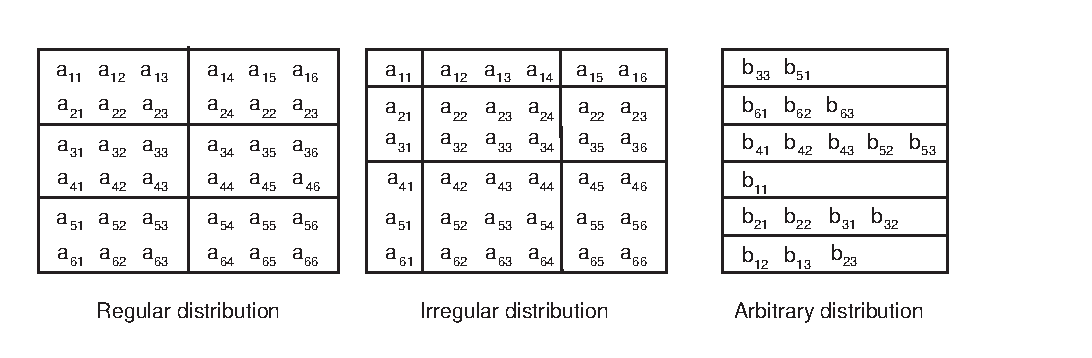
\includegraphics{GridDecomps}}
\caption{Examples of regular and irregular decomposition of
a grid {\bf a} that is 6x6, and an arbitrary decomposition of
a grid {\bf b} that is 6x3.}
\label{fig:GridDecomps}
\end{figure}

A distribution can also be specified using the DistGrid, by passing
object into a Grid create call.

\subsubsection{Grid Coordinates}
\label{sec:coordspec}
Grid Tiles can have uniform, rectilinear, or curvilinear
coordinates.  The coordinates of {\bf uniform} grids are equally spaced along
their axes, and can be fully specified by the coordinates of the two opposing points
that define the grid's physical span.  The coordinates of {\bf rectilinear} grids
are unequally spaced along their axes, and can be fully specified by giving
the spacing of grid points along each axis.  The coordinates of {\bf curvilinear 
grids} must be specified by giving the explicit set of coordinates for each
grid point.  Curvilinear grids are often uniform or rectilinear grids that 
have been warped; for example, to place a pole over a land mass so that it
does not affect the computations performed on an ocean model grid.  Figure
\ref{fig:LogRectGrids} shows examples of each type of grid.

%Any of these logically rectangular grid types can be combined through edge
%connections to form a mosaic.  Cubed sphere and yin-yang grids are examples
%of mosaic grids.  Note that as of v5.2.0 multi-tile grids have not yet been
%implemented.
 
\begin{figure}
\scalebox{0.9}{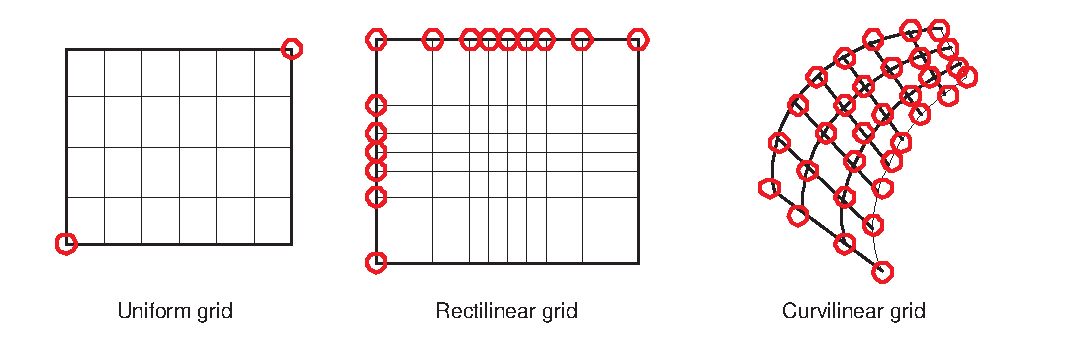
\includegraphics{LogRectGrids}}
\caption{Types of logically rectangular grid tiles.  Red circles show the
values needed to specify grid coordinates for each type.}
\label{fig:LogRectGrids}
\end{figure}

Each of these coordinate types can be set for each of the standard grid shapes
described in section \ref{sec:ShapeShortcut}.  

The table below shows how examples of common single Tile grids fall 
into this shape and coordinate taxonomy.  Note that any
of the grids in the table can have a regular or arbitrary distribution.

\medskip
\begin{tabular}{|p{.8in}|p{1.6in}|p{1.6in}|p{1.6in}|}
\hline
 & {\bf Uniform} & {\bf Rectilinear} & {\bf Curvilinear} \\ 
\hline
{\bf Sphere} & Global uniform lat-lon grid & Gaussian grid & Displaced pole grid \\
\hline
{\bf Rectangle} & Regional uniform lat-lon grid & Gaussian grid section & Polar stereographic grid section\\
\hline
\end{tabular}

\subsubsection{Coordinate Specification and Generation}

There are two ways of specifying coordinates in ESMF.  The
first way is for the user to {\bf set} the coordinates.  The second 
way is to take a shortcut and have the framework {\bf generate}
the coordinates.  

No ESMF generation routines are currently available.

See Section~\ref{sec:usage:staggerloc} for more description and examples of
setting coordinates.

\subsubsection{Staggering}

{\bf Staggering} is a finite difference technique in which the values 
of different physical quantities are placed at different locations
within a grid cell. 

The ESMF Grid class supports a variety of stagger locations, including
cell centers, corners, and edge centers. The default stagger location in 
ESMF is the cell center, and cell counts in Grid are based on this assumption.
Combinations of the 2D ESMF stagger locations are sufficient to specify any of the
Arakawa staggers.  ESMF also supports staggering in 3D and higher dimensions.
There are shortcuts for standard staggers, and interfaces through which users 
can create custom staggers.  

As a default the ESMF Grid class provides symmetric staggering, so
that cell centers are enclosed by cell perimeter (e.g. corner) 
stagger locations. This means the coordinate arrays for stagger
locations other than the center will have an additional element of 
padding in order to enclose the cell center locations.
However, to achieve other types of staggering, the user may alter 
or eliminate this padding by using the appropriate options when adding
coordinates to a Grid. 
 
In the current release, only the cell center stagger location is supported for an
arbitrarily distributed grid. For examples and a full description of the stagger interface 
see Section~\ref{sec:usage:staggerloc}. 

\subsubsection{Masking}

Masking is the process whereby parts of a grid can be marked to be
ignored during an operation, such as regridding.  Masking can be
used on a source grid to indicate that certain portions of the grid
should not be used to generate regridded data.  This is useful, for
example, if a portion of the source grid contains unusable values.
Masking can also be used on a destination grid to indicate that the
portion of the field built on that part of the Grid should not
receive regridded data.  This is useful, for example, when part of
the grid isn't being used (e.g. the land portion of an ocean grid).

ESMF regrid currently supports masking for Fields built on
structured Grids and element masking for Fields built on
unstructured Meshes. The user may mask out points in the source
Field or destination Field or both. To do masking the user sets
mask information in the Grid (see \ref{sec:usage:items}) or Mesh 
(see \ref{sec:mesh:mask}) upon which the Fields passed into the
{\tt ESMF\_FieldRegridStore()} call are built. The {\tt srcMaskValues} 
and {\tt dstMaskValues} arguments to that
call can then be used to specify which values in that mask
information indicate that a location should be masked out. For
example, if {\tt dstMaskValues} is set to (/1,2/), then any location that
has a value of 1 or 2 in the mask information of the Grid or Mesh
upon which the destination Field is built will be masked out.

Masking behavior differs slightly between regridding methods. For
non-conservative regridding methods (e.g. bilinear or high-order
patch), masking is done on points. For these methods, masking a
destination point means that that point won't participate in
regridding (e.g. won't be interpolated to). For these methods,
masking a source point means that the entire source cell using
that point is masked out. In other words, if any corner point
making up a source cell is masked then the cell is masked. For
conservative regridding methods (e.g. first-order conservative)
masking is done on cells. Masking a destination cell means that
the cell won't participate in regridding (e.g. won't be
interpolated to). Similarly, masking a source cell means that the
cell won't participate in regridding (e.g. won't be interpolated
from).  For any type of interpolation method (conservative or
non-conservative) the masking is set on the location upon
which the Fields passed into the regridding call are built.
For example, if Fields built on  {\tt ESMF\_STAGGERLOC\_CENTER} are
passed into the {\tt ESMF\_FieldRegridStore()} call then the masking
should also be set on {\tt ESMF\_STAGGERLOC\_CENTER}.
